\chapter{Potentiel électrique}


\section{Énergie potentielle électrique}

\marginpar{Tremblay \S 4.1}

\paragraph{Objectif}

\begin{enumerate}
  \item L'étudiant pourra calculer le travail fait par une force électrique.
  \item L'étudiant saura comment démontrer que la force électrique est une
    force conservative.
  \item L'étudiant pourra calculer l'énergie potentielle électrique et sera en
    mesure d'expliquer le lien entre la force et l'énergie potentielle.
\end{enumerate}



\subsection*{Exercice de rappel sur la notion de travail}

\marginpar{Diapo}
\marginpar{10 minutes}

Classez les situations suivantes en ordre croissant du travail fait par la
force électrique sur la charge $q > 0$.

\begin{center}
  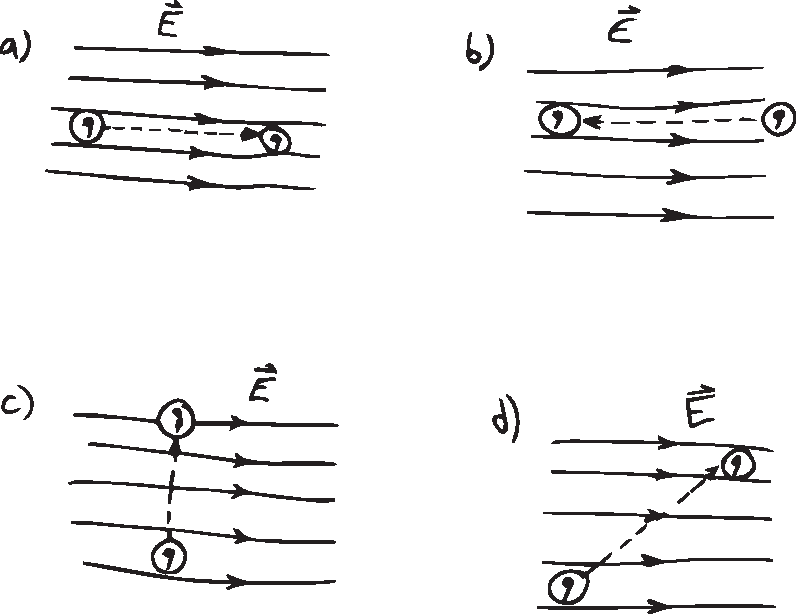
\includegraphics[scale=0.7]{04-potentiel/figures/travail-force-electrique.pdf}
\end{center}

\textit{Solution}: $W_b < W_c < W_a = W_d$


\subsection*{Le travail fait par une force électrique}

\marginpar{10 minutes}

On considère une région d'espace avec un champ électrique $\vec{E}$. Une charge
ponctuelle $q$ dans cette région subit une force électrique $\vec{F} =
q\vec{E}$. Si la particule se déplace du point $A$ au point $B$, le travail
effectué par la force électrique est
\[
  W = \int_A^B \vec{F} \cdot d\vec{s}
\]
où $d\vec{s}$ est une petite partie du chemin parcouru. Dans le cas simple où
la trajectoire est une ligne droite de longueur $L$ et le champ électrique est
uniforme
\[
  W = FL.
\]
On peut récrire l'expression du travail en terme du champ électrique
\[
  W = q \int_A^B \vec{E}\cdot d\vec{s}
\]
\begin{center}
  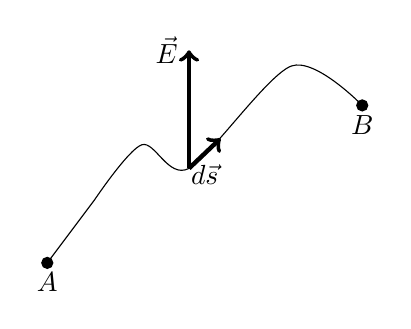
\begin{tikzpicture}
    \coordinate (A) at (0, 0);
    \coordinate (B) at (4, 2);
    \draw[fill=black] (A) circle (2pt);
    \draw[fill=black] (B) circle (2pt);
    \node[below] (nA) at (A) {$A$};
    \node[below] (nB) at (B) {$B$};
    \draw (A) -- plot[smooth] coordinates {(0.6, 0.8) (1.2, 1.5) (1.8, 1.2) (3.1, 2.5) (B)};
    \draw[ultra thick, ->] (1.8, 1.2) -- node[below] {$d\vec{s}$} (2.2, 1.58);
    \draw[ultra thick, ->] (1.8, 1.2) -- ++(0, 1.5) node[left] {$\vec{E}$};
  \end{tikzpicture}
\end{center}


\subsection*{Est-ce que la force électrique est conservative?}

\marginpar{Diapo}
\marginpar{15 minutes}

Une particule de déplace de l'origine $\vec{r}_0 = \vecxyz{0}{0}{0}$ jusqu'au
point $\vec{r} = \vecxyz{a}{b}{c}$ dans un champ électrique constant $\vec{E} =
E_z \zhat$ où $E_z$ est constant.  Déterminer le travail fait par la force
électrique pour les deux trajectoires suivantes.

\begin{itemize}
  \item Le long de la ligne droite qui relie $\vec{r}_0$ à $\vec{r}$.
  \item Le long de la ligne qui va de $\vec{r}_0$ à $\vecxyz{a}{b}{0}$, puis le
    long de la ligne qui va de $\vecxyz{a}{b}{0}$ à $\vecxyz{a}{b}{c}$.
\end{itemize}

\begin{description}
  \item[Le long de la ligne droite qui relie $(0,0,0)$ à $(a,b,c)$.]

    L'angle entre le champ électrique et le déplacement est constant sur toute
    la trajectoire :
    \[
      \cos \theta = \frac{c}{\sqrt{a^2 + b^2 + c^2}}.
    \]
    Le travail fait par la force électrique est donc
    \begin{align*}
      W &= \int_{(0,0,0)}^{(a,b,c)} E_z \cos \theta \, ds \\
        &= E_z \cos \theta \int_{(0,0,0)}^{(a,b,c)}\, ds \\
        &= E_z c,
    \end{align*}
    c'est-à-dire que le travail de la force électrique est déterminé par la
    composante du déplacement qui est parallèle au champ. Ceci ne devrait pas
    être une surprise.

  \item[Le long de la droite $(0,0,0)$ à $(a,b,0)$, puis le long de la droite
    $(a,b,0)$ à $(a,b,c)$.]

    Dans la première partie de la trajectoire, le déplacement est
    perpendiculaire au champ électrique, donc le travail effectué par la force
    électrique est nul. Pour la seconde partie de la trajectoire, le
    déplacement est parallèle au champ, le travail est donc  $E_z c$. Le
    travail total est donc encore $E_z c$.
\end{description}


\subsection*{Indépendance du chemin}

\marginpar{5 minutes}

L'exemple précédent suggère que le travail fait par la force électrique est
indépendant du chemin. Il est possible de montrer que c'est le cas, peu importe
le chemin choisi.

Une force pour laquelle le travail est indépendant du chemin est
\textbf{conservative}.

Rappelez-vous le cas de la force gravitationnelle à la surface de la Terre (ici
l'axe $y$ pointe vers le haut)
$$W_g = -mg \Delta y$$


\subsection*{Énergie potentielle électrique}

\marginpar{10 minutes}

Puisque la force électrique est conservative, on peut lui associer une énergie
potentielle. On définit l'énergie potentielle électrique de la même façon que
nous avons défini l'énergie potentielle gravitationnelle: c'est l'opposé du
travail fait par la force,
$$\Delta U = -W$$
ie,
\[
  \Delta U = - q\int_A^B \vec{E} \cdot d\vec{s}
\]


\subsection*{Exemple}

\marginpar{40 minutes}
\marginpar{Diapo}

On considère une mince tige métallique cylindrique très longue portant une
charge uniforme.  La densité linéique de charge est de $\lambda =
\SI{0.948}{\micro\coulomb\per\meter}$. Un électron est relâché \SI{35}{mm}
de la tige.

\begin{enumerate}
  \item Calculer la variation d'énergie potentielle du système après que
    l'électron se soit déplacé de \SI{1}{cm}.
  \item Si l'électron était initialement au repos, déterminer sa vitesse à la
    fin de son déplacement.
  \item Tracer un graphique du module du champ électrique généré par la tige en
    fonction de la distance par rapport à son axe.
  \item Tracer un graphique de l'énergie potentielle de l'électron en fonction
    de sa distance par rapport à l'axe de la tige.
\end{enumerate}

\paragraph{Solution}

\begin{center}
  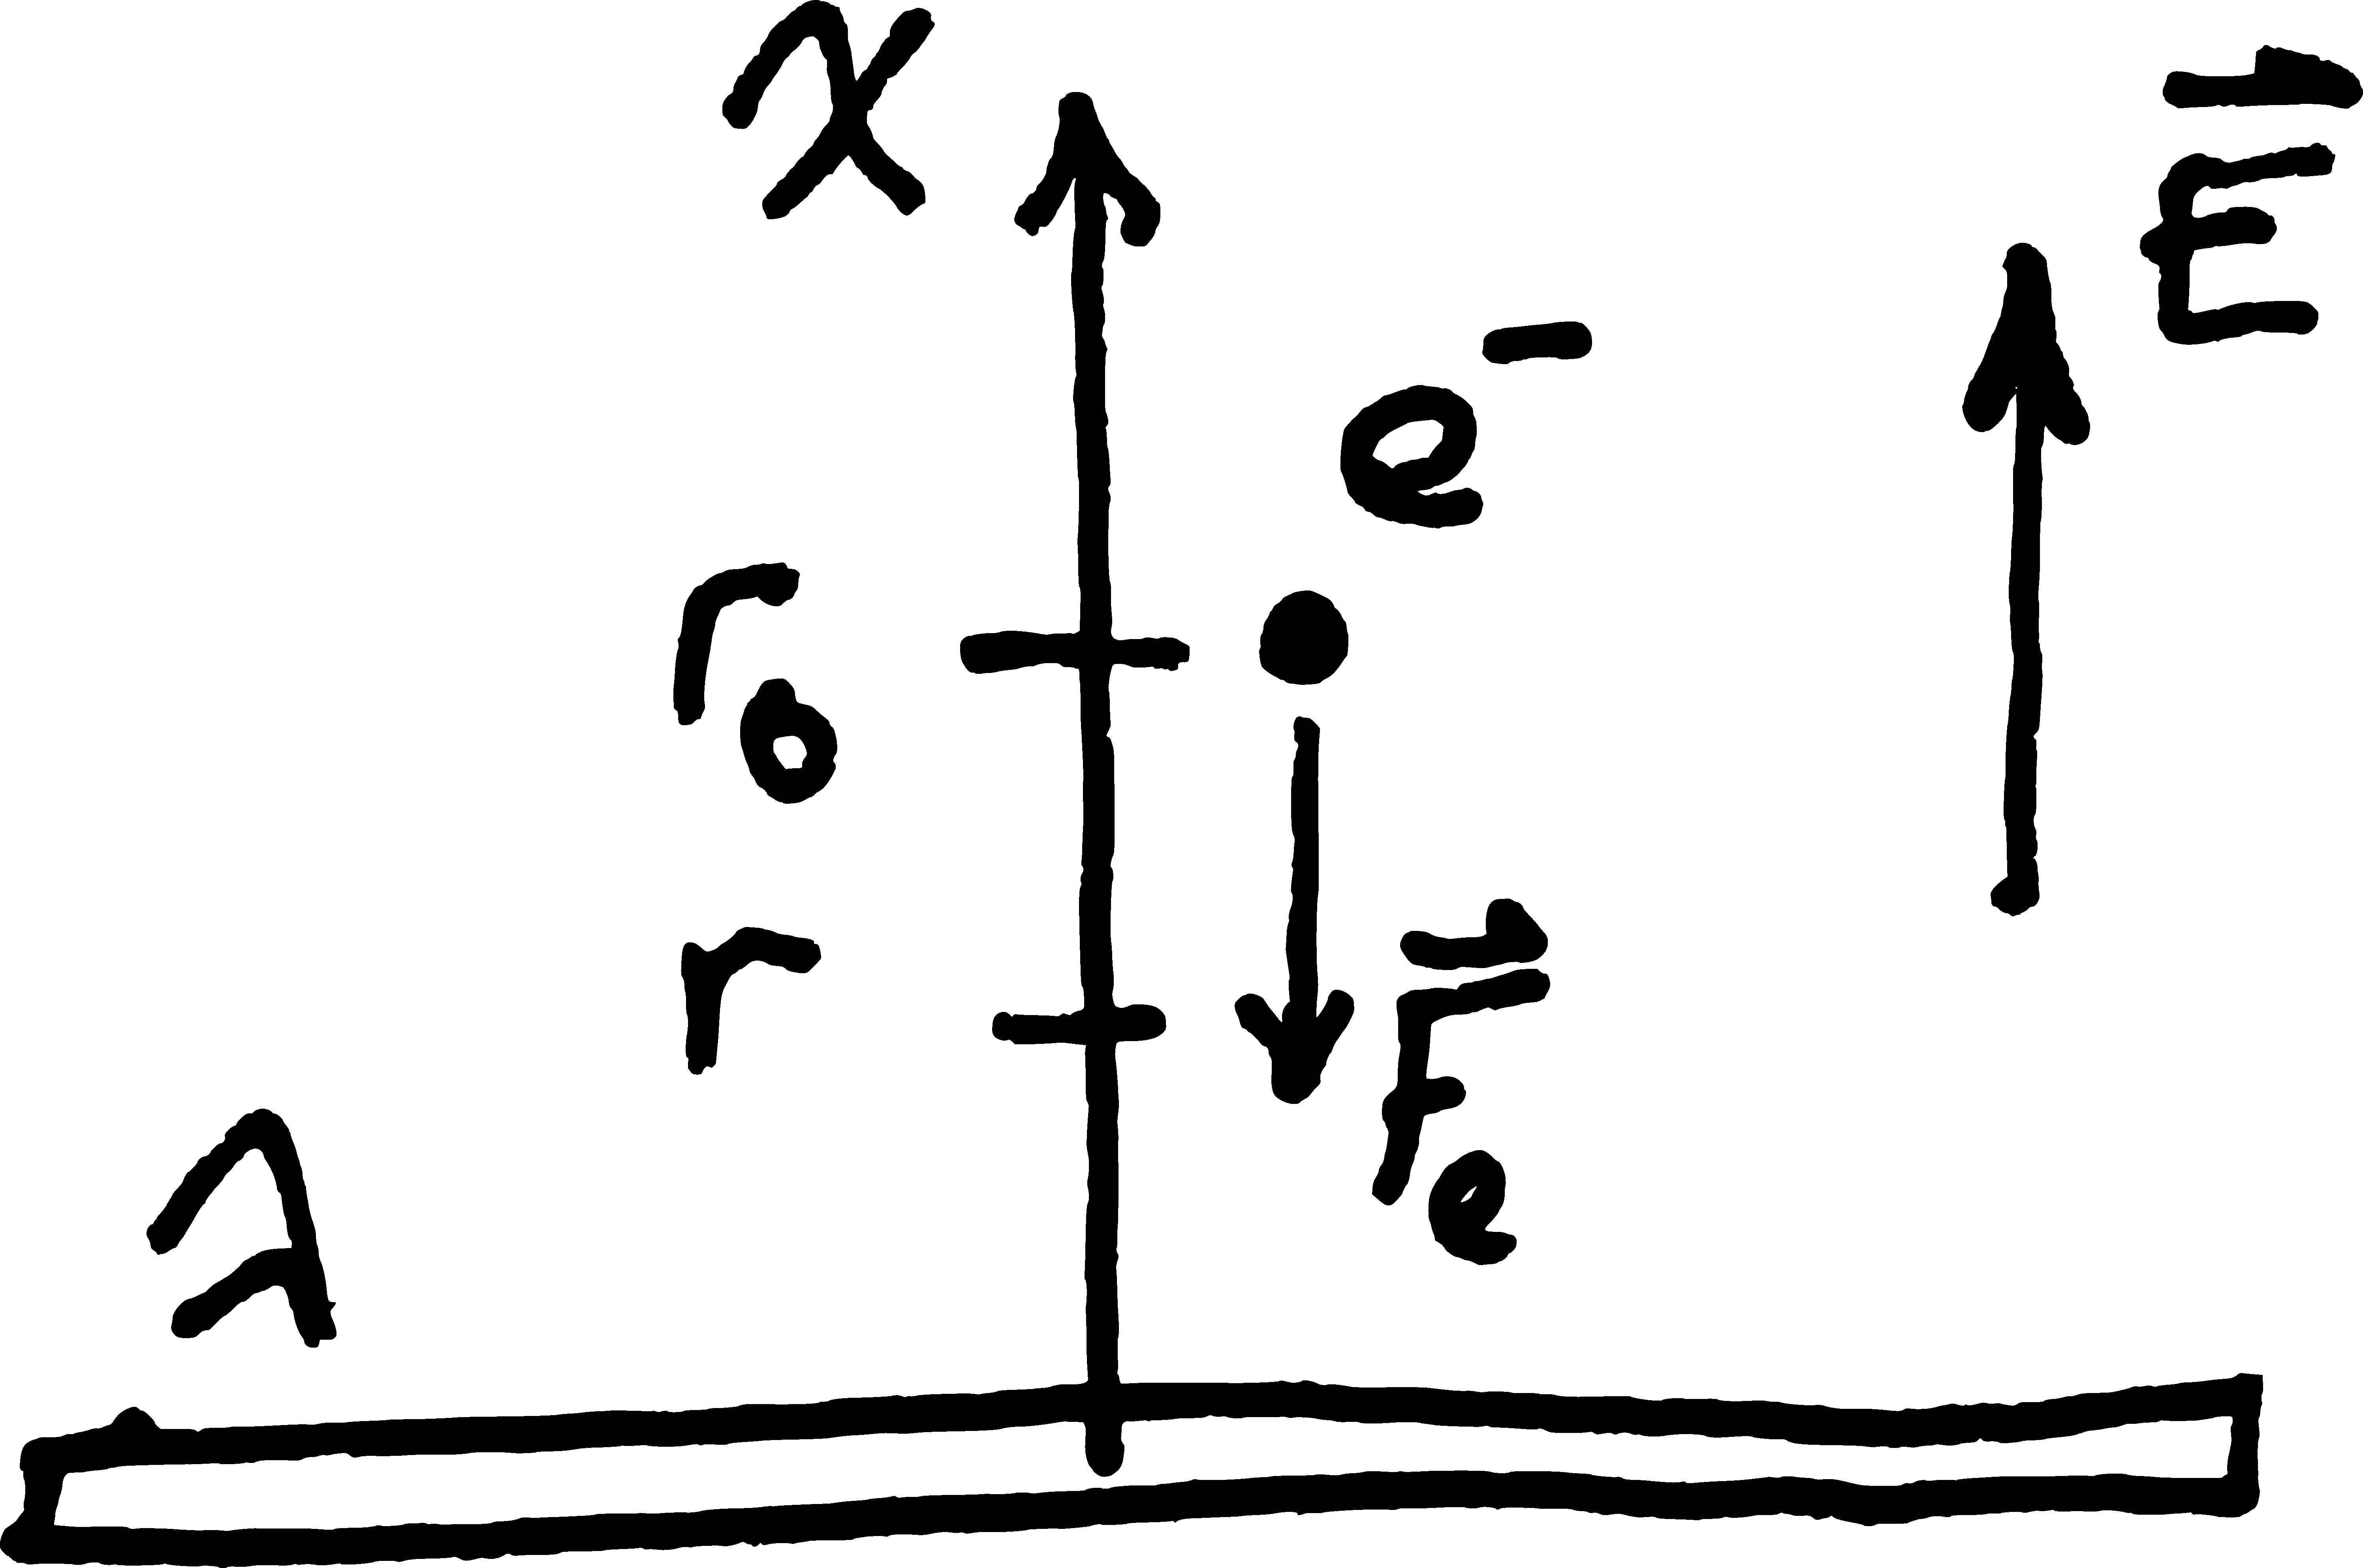
\includegraphics[scale=0.04]{04-potentiel/figures/exercice-tige-energie-potentielle.pdf}
\end{center}
\begin{enumerate}
    \item L'électron est attiré par la tige chargée positivement, donc il se
        rapproche de la tige. Le champ électrique de la tige est celui d'un fil
        infini soit
        \[\vE = \frac{2k\lambda}{x} \xhat.\]
        On peut donc calculer la différence d'énergie potentielle
        \begin{align*}
            \Delta U &= -q \int_{r_0}^{r} \frac{2k\lambda}{x} \xhat \cdot d\vec{s} \\
                     &= -2k\lambda q \int_{r_0}^r \frac{1}{x} \xhat \cdot (dx \xhat
                        + dy \yhat + dz \zhat) \\
                     &= -2k\lambda q \int_{r_0}^r \frac{1}{x} dx \\
                     &= -2k\lambda q \left[ \ln(r) - \ln(r_0) \right] \\
                     &= -2k\lambda q \ln\left( \frac{r}{r_0} \right) \\
                     &= 2k\lambda e  \ln\left( \frac{r}{r_0} \right) \\
                     &= \SI{-9.186e-16}{J}
        \end{align*}
    \item Au départ, son énergie cinétique était nulle car il était immobile,
        par conséquent
        \begin{align*}
            \Delta K = K_f - K_i = K_f.
        \end{align*}
        Par le principe de conservation de l'énergie mécanique
        \begin{align*}
            \Delta K + \Delta U &= 0 \\
            \Delta K &= -\Delta U \\
            \frac{1}{2} m_e v^2 &= -\Delta U \\
            v &= \sqrt{\frac{-2\Delta U}{m_e}} \\
            v &= \SI{4.491e7}{m/s}
        \end{align*}
        Donc
        \[\vec{v} = -\SI{4.491e7}{m/s} \xhat\]
    \item Les graphiques du module du champ magnétique et de l'énergie
        potentielle sont ci-dessous.

      \begin{center}
        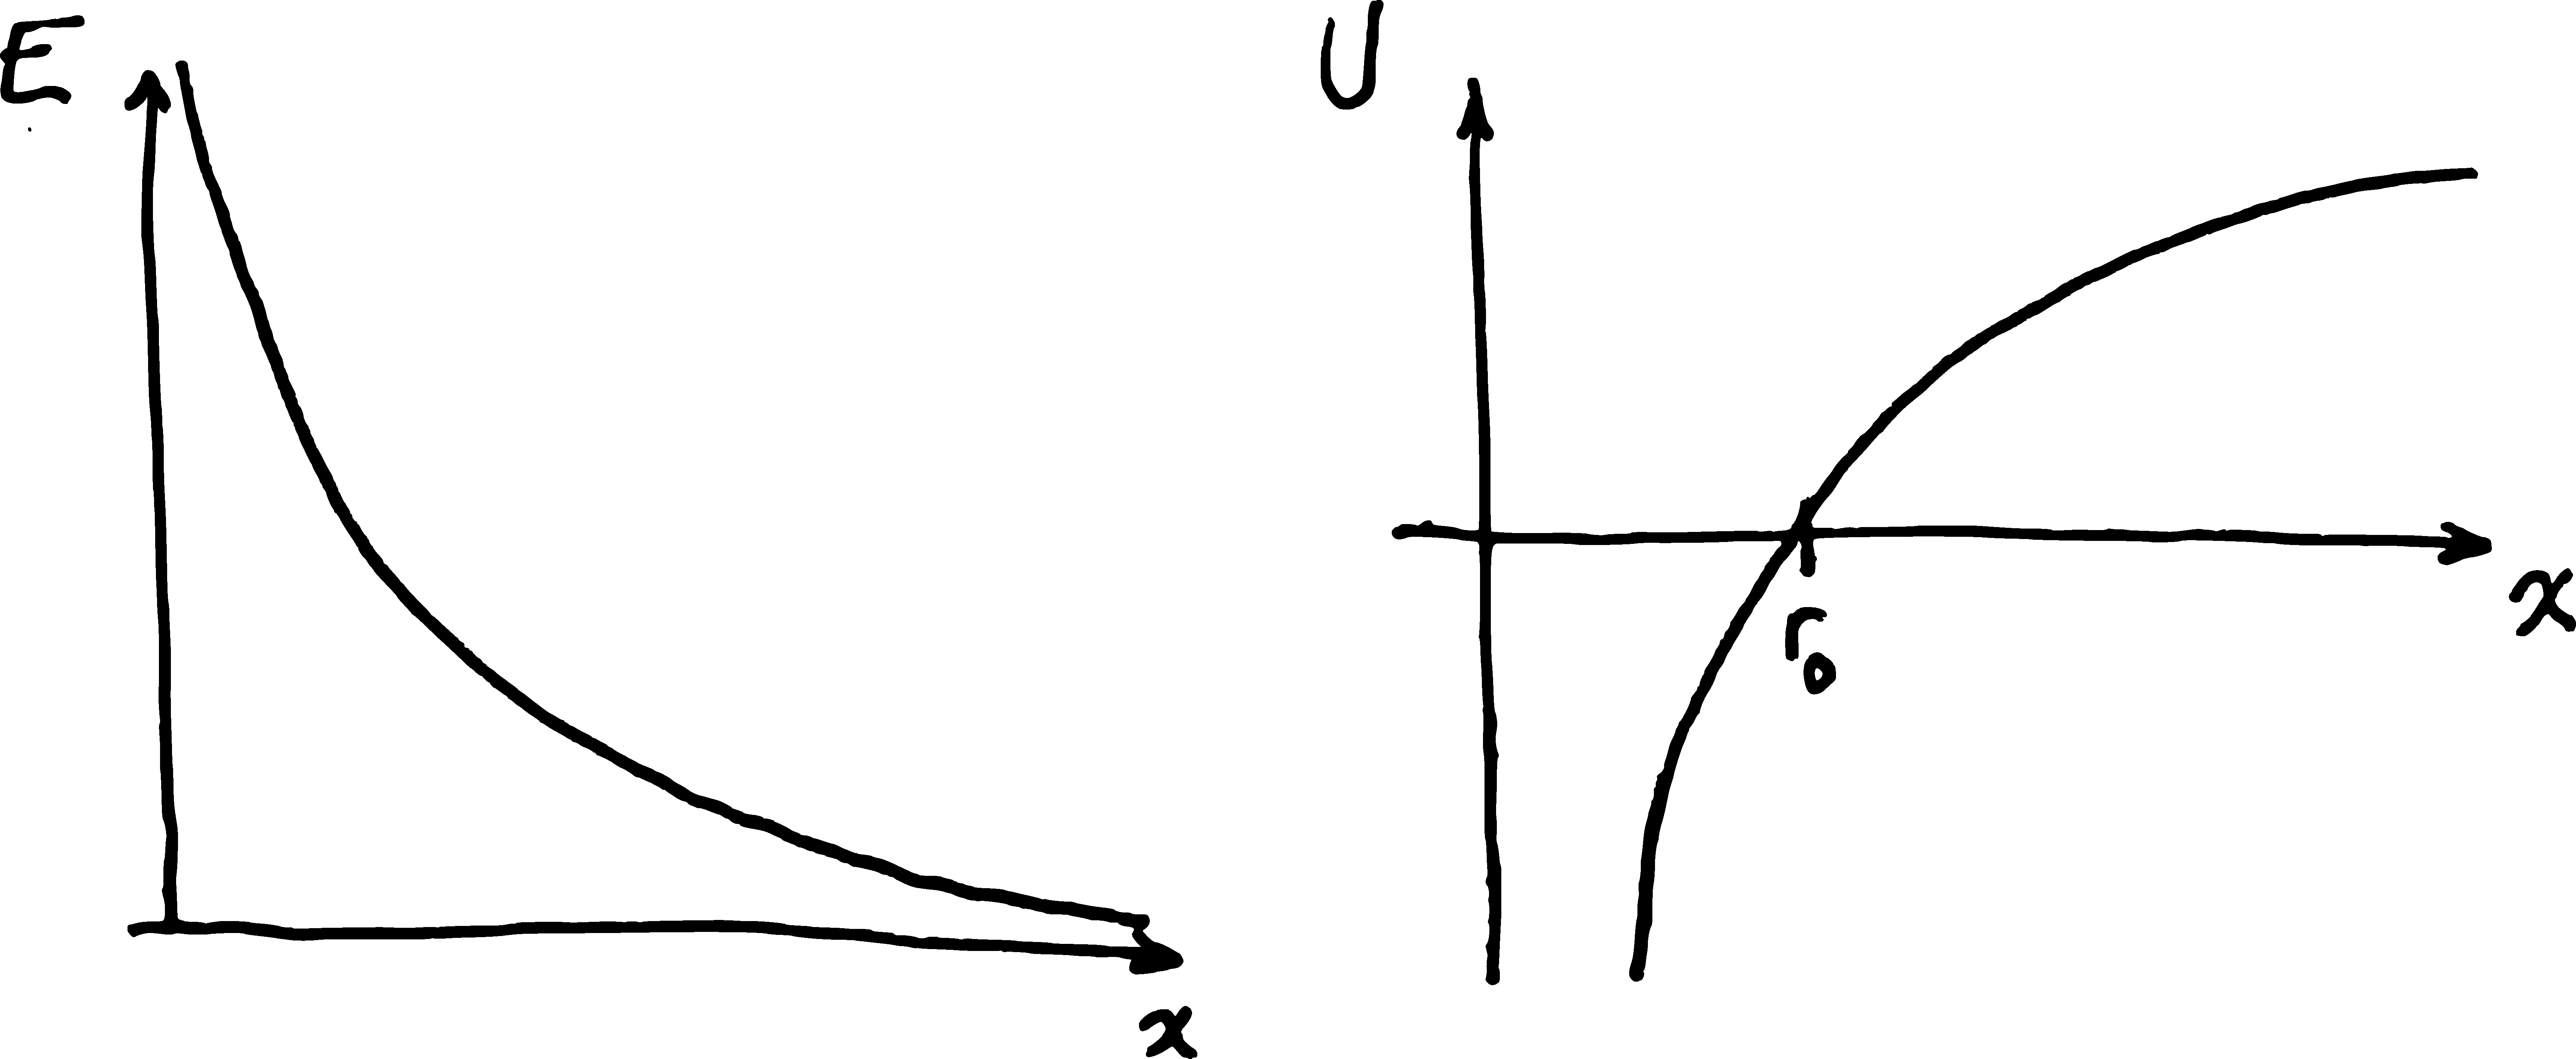
\includegraphics[scale=0.09]{04-potentiel/figures/exercice-tige-energie-potentielle-graphiques.pdf}
      \end{center}
\end{enumerate}


\sectionline


\section{Potentiel électrique}

\marginpar{Tremblay \S 4.2}

\paragraph{Objectif}

\begin{enumerate}
  \item L'étudiant comprendra les concepts de potentiel électrique et de
    différence de potentiel. Il pourra expliquer le lien entre le potentiel et
    le champ électrique.
\end{enumerate}



\subsection*{La différence de potentiel électrique}

\marginpar{10 minutes}

Dans la formule pour l'énergie potentielle électrique
\[
  \Delta U = -q \int_A^B \vec{E}\cdot d\vec{s},
\]
on remarque que l'intégrale ne dépend pas du tout de la charge qui se déplace.
L'intégrale dépend uniquement de la source du champ électrique. Comme nous
l'avions fait avec la force et le champ électrique, nous pouvons définir une
quantité qui ne dépend que de la source
\[
  \Delta V = - \int_A^B \vec{E}\cdot d\vec{s}.
\]
Cette quantité s'appelle une \textbf{différence de potentiel électrique}.

Les unités de la différence de potentiel sont les volts
$$\SI{1}{V} = \SI{1}{Nm/C}$$

On exprime souvent le champ électrique en \si{\volt\per\meter}.

Si une particule chargée $q$ se déplace entre deux points séparés par une
différence de potentiel $\Delta V$, sont énergie potentielle varie de
\[
  \Delta U = q \Delta V
\]


\subsection*{Exemple}

\marginpar{10 minutes}
\marginpar{Diapo}
Deux grandes plaques métalliques sont maintenues à une différence de potentiel
de \SI{12}{V}. Elles sont séparées d'une distance de \SI{1}{cm}. Un électron
qui se trouve juste à côté d'une des plaques se déplace jusqu'à l'autre plaque.
Si l'électron est initialement immobile, déterminer le module de sa vitesse
lorsqu'il atteint l'autre plaque.

\begin{center}
  \begin{tikzpicture}
    \draw[very thick] (0, 0) -- (0, 2);
    \draw[very thick] (4, 0) -- (4, 2);
    \foreach \y in {0.25, 0.75, ..., 1.9} {
      \node at (-0.3, \y) {$+$};
      \node at (4.3, \y) {$-$};
    }
    \fill (3.8, 1) circle (0.1);
    \node at (3.75, 0.6) {$e^{-}$};
    \draw[->] (3.65, 1) -- ++(-1, 0);
  \end{tikzpicture}
\end{center}

L'énergie cinétique initiale est de $0$ car l'électron est au repos. La
variation d'énergie potentielle lorsque l'électron passe de la plaque négative
à la plaque positive est de
\begin{align*}
  \Delta U &= q \Delta V \\
           &= -e \Delta V
\end{align*}
où $\Delta V = \SI{12}{V}$. Par le principe de conservation de l'énergie
mécanique, on a
\begin{align*}
  \Delta K + \Delta U &= 0  \\
      K_f - e\Delta V &= 0  \\
      K_f &= e\Delta V     \\
      K_f &= e \cdot \SI{12}{V}  \\
      K_f &= \SI{12}{eV}   \\
        v &= \sqrt{\frac{2 \cdot \SI{12}{eV}}{m}}  \\
        v &= \SI{2.055e6}{m/s}
\end{align*}


\subsection*{Électron-volt pour mesurer l'énergie}

\marginpar{5 minutes}

L'\textbf{électron-volt} (\si{eV}) est une unité de mesure d'énergie. Un
\si{eV} correspond à l'énergie cinétique que va acquérir un électron accéléré
dans une différence de potentiel de \SI{1}{V}.

\[
    \SI{1}{eV} = \SI{1.602e-19}{J}
\]


\subsection*{Exemple}

\marginpar{10 minutes}
\marginpar{Diapo}

Deux grandes plaques métalliques sont maintenues à une différence de potentiel
de \SI{12}{V}. On augmente la distance entre les plaques. Expliquez ce qui doit
se produire avec la densité surfacique de charge sur les plaques pour que la
différence de potentiel demeure constante.

\begin{center}
  \begin{tikzpicture}
    \draw[very thick] (0, 0) -- (0, 2);
    \draw[very thick] (4, 0) -- (4, 2);
    \node at (-0.5, 2.2) {$+\sigma$};
    \node at (4.5, 2.2) {$-\sigma$};
    \foreach \y in {0.25, 0.75, ..., 1.9} {
      \draw[->] (0.2, \y) -- (3.8, \y);
    }
    \node at (2, 1) {$\vE$};
    \draw[->] (-0.5, -0.5) -- (4.5, -0.5) node[below] {$x$};
  \end{tikzpicture}
\end{center}

Le champ généré par chaque plaque entre les plaques est
\begin{align*}
  E_{+} = \frac{\sigma}{2 \varepsilon_0} \quad\quad E_{-} = \frac{\sigma}{2 \varepsilon_0}
\end{align*}
donc le champ total entre les plaques est constant de grandeur
\[
  E = \frac{\sigma}{\epsilon_0}.
\]
Si on va d'un point $x_0$ à un point $x$, la différence de potentiel est
\begin{align*}
  \Delta V &= - \int_{x_0}^x \vE \cdot d\vec{s}  \\
           &= - \int_{x_0}^x E dx  \\
           &= - E\int_{x_0}^x dx  \\
           &= - E (x - x_0) \\
           &= - \frac{\sigma}{\varepsilon_0} (x - x_0) \\
\end{align*}
En particulier, si on va de la plaque négative à la plaque positive,
\[\Delta V = \frac{\sigma d}{\varepsilon_0} \]
donc, si la ddp est constante et que la distance entre les plaques augmente,
la densité surfacique de charge doit diminuer.



\subsection*{Potentiel électrique d'une charge ponctuelle}

Pour une charge ponctuelle
\[
  E_r = \coulombcst \frac{q}{r^2}.
\]
La différence de potentiel entre deux points $A$ et $B$ est donc
\begin{align*}
  \Delta V &= -\int_A^B \vec{E}\cdot d\vec{s} \\
    &= -\int_{r_A}^{r_B} \coulombcst \frac{q}{r^2} \,dr \\
    &= -kq \int_{r_A}^{r_B} \frac{1}{r^2} \,dr \\
    &= -kq \left[ \frac{-1}{r} \right]_{r_A}^{r_B} \\
    &= \frac{kq}{r_B} - \frac{kq}{r_A} \\
    &= V_B - V_A
\end{align*}
donc
$$V = \frac{kq}{r}$$


\sectionline


\subsection*{Travail personnel}

Faire les numéros 1, 2, 4, 10 et 22 du livre et les remettre avant de partir.


\sectionline


\subsection*{Rappels}

On a vu que le potentiel, l'énergie potentielle, la force et le champ
électrique sont reliés:

\begin{align*}
  \vF &= q\vE  \\
  \Delta U &= -\int_A^B \vF \cdot d\vec{s} = q \Delta V \\
  \Delta V &= -\int_A^B \vE \cdot d\vec{s} = \Delta U / q
\end{align*}

\begin{center}
\begin{tabular}{p{4cm}llp{4cm}}
  \toprule
  Objet    &     $\vE$      &   $V$     &  Notes  \\
  \midrule
  Charge ponctuelle $q$  &
      $\displaystyle{\frac{kq}{r^2} \vec{u}_r}$  &
      $\displaystyle{\frac{kq}{r}}$  &
      Potentiel nul à l'infini   \\[10pt]
  Tige infinie (au-dessus de l'axe)  &
      $\displaystyle{\frac{2k \lambda}{r}}\vec{u}_r$  &
      $\displaystyle{-2k \lambda \ln \left( \frac{r}{r_0} \right)}$  &
      Potentiel nul à la position initiale  \\[10pt]
  Plan infini  &
      $\displaystyle{\frac{\sigma}{2\varepsilon_0}\zhat}$  &
      $\displaystyle{\pm Ed}$  &
      Potentiel nul à la position initiale  \\[10pt]
  \bottomrule
\end{tabular}
\end{center}

Si on a une expression pour le potentiel, on peut facilement déterminer la
différence de potentiel entre deux points quelconques en calculant
\[\Delta V = V_f - V_i.\]



\subsection*{Exercice: potentiel d'une sphère conductrice}

Tracer le potentiel en fonction de la distance pour une sphère conductrice
chargée de rayon $R$ portant une charge $Q$.



\section{Potentiel d'un ensemble de charges}

\marginpar{Tremblay \S 4.3}

Le principe de superposition s'applique au potentiel électrique :
le potentiel d'un ensemble de charges est la somme des potentiels.

On peut utiliser ce principe pour calculer le potentiel de n'importe quel objet
chargé :
\[
  V = \int_\text{objet} \frac{k dq}{r}.
\]


%\subsection*{Potential of a Ring of Charge}

%Consider a charged ring or radius $R$ and total charge $q$.  Determine the
%electric potential a distance $d$ from the center of the ring on the axis
%perpendicular to the plane of the ring.

%There are two ways to proceed: use the potential of a point charge and
%integrate or use the electric field of a ring.

%\paragraph{With Potential of Point Charge}
%The ring can be thought of a collection of point charges.  Each line element
%of the ring produces a potential
%\[
  %dV = \coulombcst \frac{dq}{r}
%\]
%where $r = \sqrt{R^2 + d^2}$.  Since all line elements are at the same
%distance from the point at which we are calculating the potential, the
%integral over the ring is easily evaluated:
%\begin{align*}
  %V &= \int_\text{ring} \coulombcst \frac{dq}{r} \\
    %&= \coulombcst \frac{1}{r} \int_\text{ring} dq \\
    %&= \coulombcst \frac{q}{\sqrt{R^2 + d^2}}
%\end{align*}

%\paragraph{With Electric Field}
%If the $z$ axis is perpendicular to the plane of the ring and passes through
%the center of the ring, the electric field of the ring is
%\[
  %\vec{E} = \coulombcst \frac{qz}{(R^2 + z^2)^{3/2}} \zhat
%\]
%Consider the trajectory that goes from infinitely far on the $z$ axis down to
%$z = d$.  The potential is then
%\begin{align*}
  %V &= -\int_\infty^d \vec{E} \cdot (\zhat \,dz) \\
    %&= -\frac{q}{4\pi\varepsilon_0} \int_\infty^d \frac{z}{(R^2 + z^2)^{3/2}} \,dz \\
    %&= -\frac{q}{4\pi\varepsilon_0} \frac{1}{2} \int_\infty^{R^2 + d^2} \frac{1}{u^{3/2}} \,du \\
    %&= \frac{q}{4\pi\varepsilon_0} \left[\frac{1}{u^{1/2}}\right]_\infty^{R^2 + d^2} \\
    %&= \coulombcst \frac{q}{\sqrt{R^2 + d^2}}
%\end{align*}


%\subsection*{Exercice}

%Calculer le potentiel électrique à une distance $D$ au dessus d'un disque
%chargé de densité surfacique $\sigma$ et de rayon $R$.

%\begin{align*}
  %V &= \int_{0}^{R} \frac{k dq}{r} \\
    %&= \int_{0}^{R} \frac{k 2\pi a da}{\sqrt{a^2 + D^2}} \\
    %&= 2\pi k\sigma \left[ \sqrt{a^2 + D^2} \right]_0^R \\
    %&= 2\pi k\sigma \left[ \sqrt{R^2 + D^2} - D \right] \\
%\end{align*}



\subsection*{Énergie potentielle électrique d'un ensemble de charges}

On considère un ensemble de $n$ charges ponctuelles $q_1, q_2, \ldots, q_n$.
Pour calculer l'énergie potentielle de cet ensemble de charges, on doit
l'assembler, une charge à la fois. Placer la première charge ne requiert aucun
travail puisque le champ électrique est nul au départ. Apporter la seconde
charge nécessite un travail puisqu'on doit la déplacer dans le champ électrique
produit par la première charge. L'énergie requise est
\[
  U_2 = q_2 V_1.
\]
Pour la troisième charge, on doit tenir compte du potentiel créé par les deux
premières charges. Puisque le potentiel respecte le principe de superposition,
on a
\[
  U_3 = q_3 V_1 + q_3 V_2 = q_3 (V_1 + V_2).
\]
On peut répéter l'argument pour les charges suivantes. On obtient l'énergie
potentielle totale du système en additionnant les énergies $U_1, U_2, \ldots,
U_n$.  La somme contient un terme pour chaque paire de charges.
\[
  U = \sum_{i < j} q_i V_j
\]



\sectionline



\subsection*{Exercice}

Quatre charges sont placées aux sommets d'un carré de côté $d = \SI{3}{cm}$. Les
charges sont de $q_1 = \SI{1.7}{\micro\coulomb}$, $q_2 = \SI{-3}{\micro\coulomb}$,
$q_3 = \SI{5}{\micro\coulomb}$ et $q_4 = \SI{-4}{\micro\coulomb}$.


\begin{itemize}
  \item Déterminer le potentiel à \SI{2}{cm} en-dessous de la charge $q_1$.
  \item Déterminer l'énergie potentielle de cette distribution de charges.
\end{itemize}

\begin{center}
  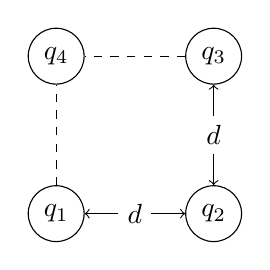
\begin{tikzpicture}
    \coordinate (p1) at (0, 0);
    \coordinate (p2) at (2, 0);
    \coordinate (p3) at (2, 2);
    \coordinate (p4) at (0, 2);
    \node[draw, circle] (q1) at (p1) {$q_1$};
    \node[draw, circle] (q2) at (p2) {$q_2$};
    \node[draw, circle] (q3) at (p3) {$q_3$};
    \node[draw, circle] (q4) at (p4) {$q_4$};
    \draw[<->] (q1) -- node[fill=white] {$d$} (q2);
    \draw[<->] (q2) -- node[fill=white] {$d$} (q3);
    \draw[dashed] (q1) -- (q4);
    \draw[dashed] (q3) -- (q4);
  \end{tikzpicture}
\end{center}

\begin{align*}
  V &= V_1 + V_2 + V_3 + V_4 \\
    &= \frac{kq_1}{r_1} + \frac{kq_2}{r_2} + \frac{kq_3}{r_3} +
    \frac{kq_4}{r_4} \\
    &= \SI{67800}{V}
\end{align*}

\begin{align*}
  U &= q_1 V_2 + q_1 V_3 + q_1 V_4 + q_2 V_3 + q_2 V_4 + q_3 V_4 \\
    &= \frac{kq_1 q_2}{d} + \frac{kq_1 q_3}{\sqrt{2}d} + \frac{kq_1 q_4}{d} +
    \frac{kq_2 q_3}{d} + \frac{kq_2q_4}{\sqrt{2} d} + \frac{kq_3q_4}{d} \\
    &= \SI{-9.71}{J}
\end{align*}



\subsection*{Surfaces équipotentielles}

Une région connexe de l'espace qui est au même potentiel électrique est appelée
une \textbf{surface équipotentielle}. Par exemple, puisque le champ électrique
à l'intérieur d'un conducteur est nul, la surface d'un conducteur est une
équipotentielle.

Les surfaces équipotentielles sont toujours perpendiculaires aux lignes de
champ électrique. En effet, si on se déplace le long d'une équipotentielle,
$\Delta V = 0$. Or,
\[
  \Delta V = - \int \vE \cdot d\vec{s}
\]
n'est égal à zéro que si l'angle entre le déplacement et le champ électrique
est nul (en supposant que le champ électrique et le déplacement ne sont pas
nuls).



\subsection*{Exercice}

\marginpar{Diapo}

On place un électron dans une région de l'espace où les surfaces
équipotentielles sont telles qu'illustrées dans le schéma ci-dessous.

\begin{center}
  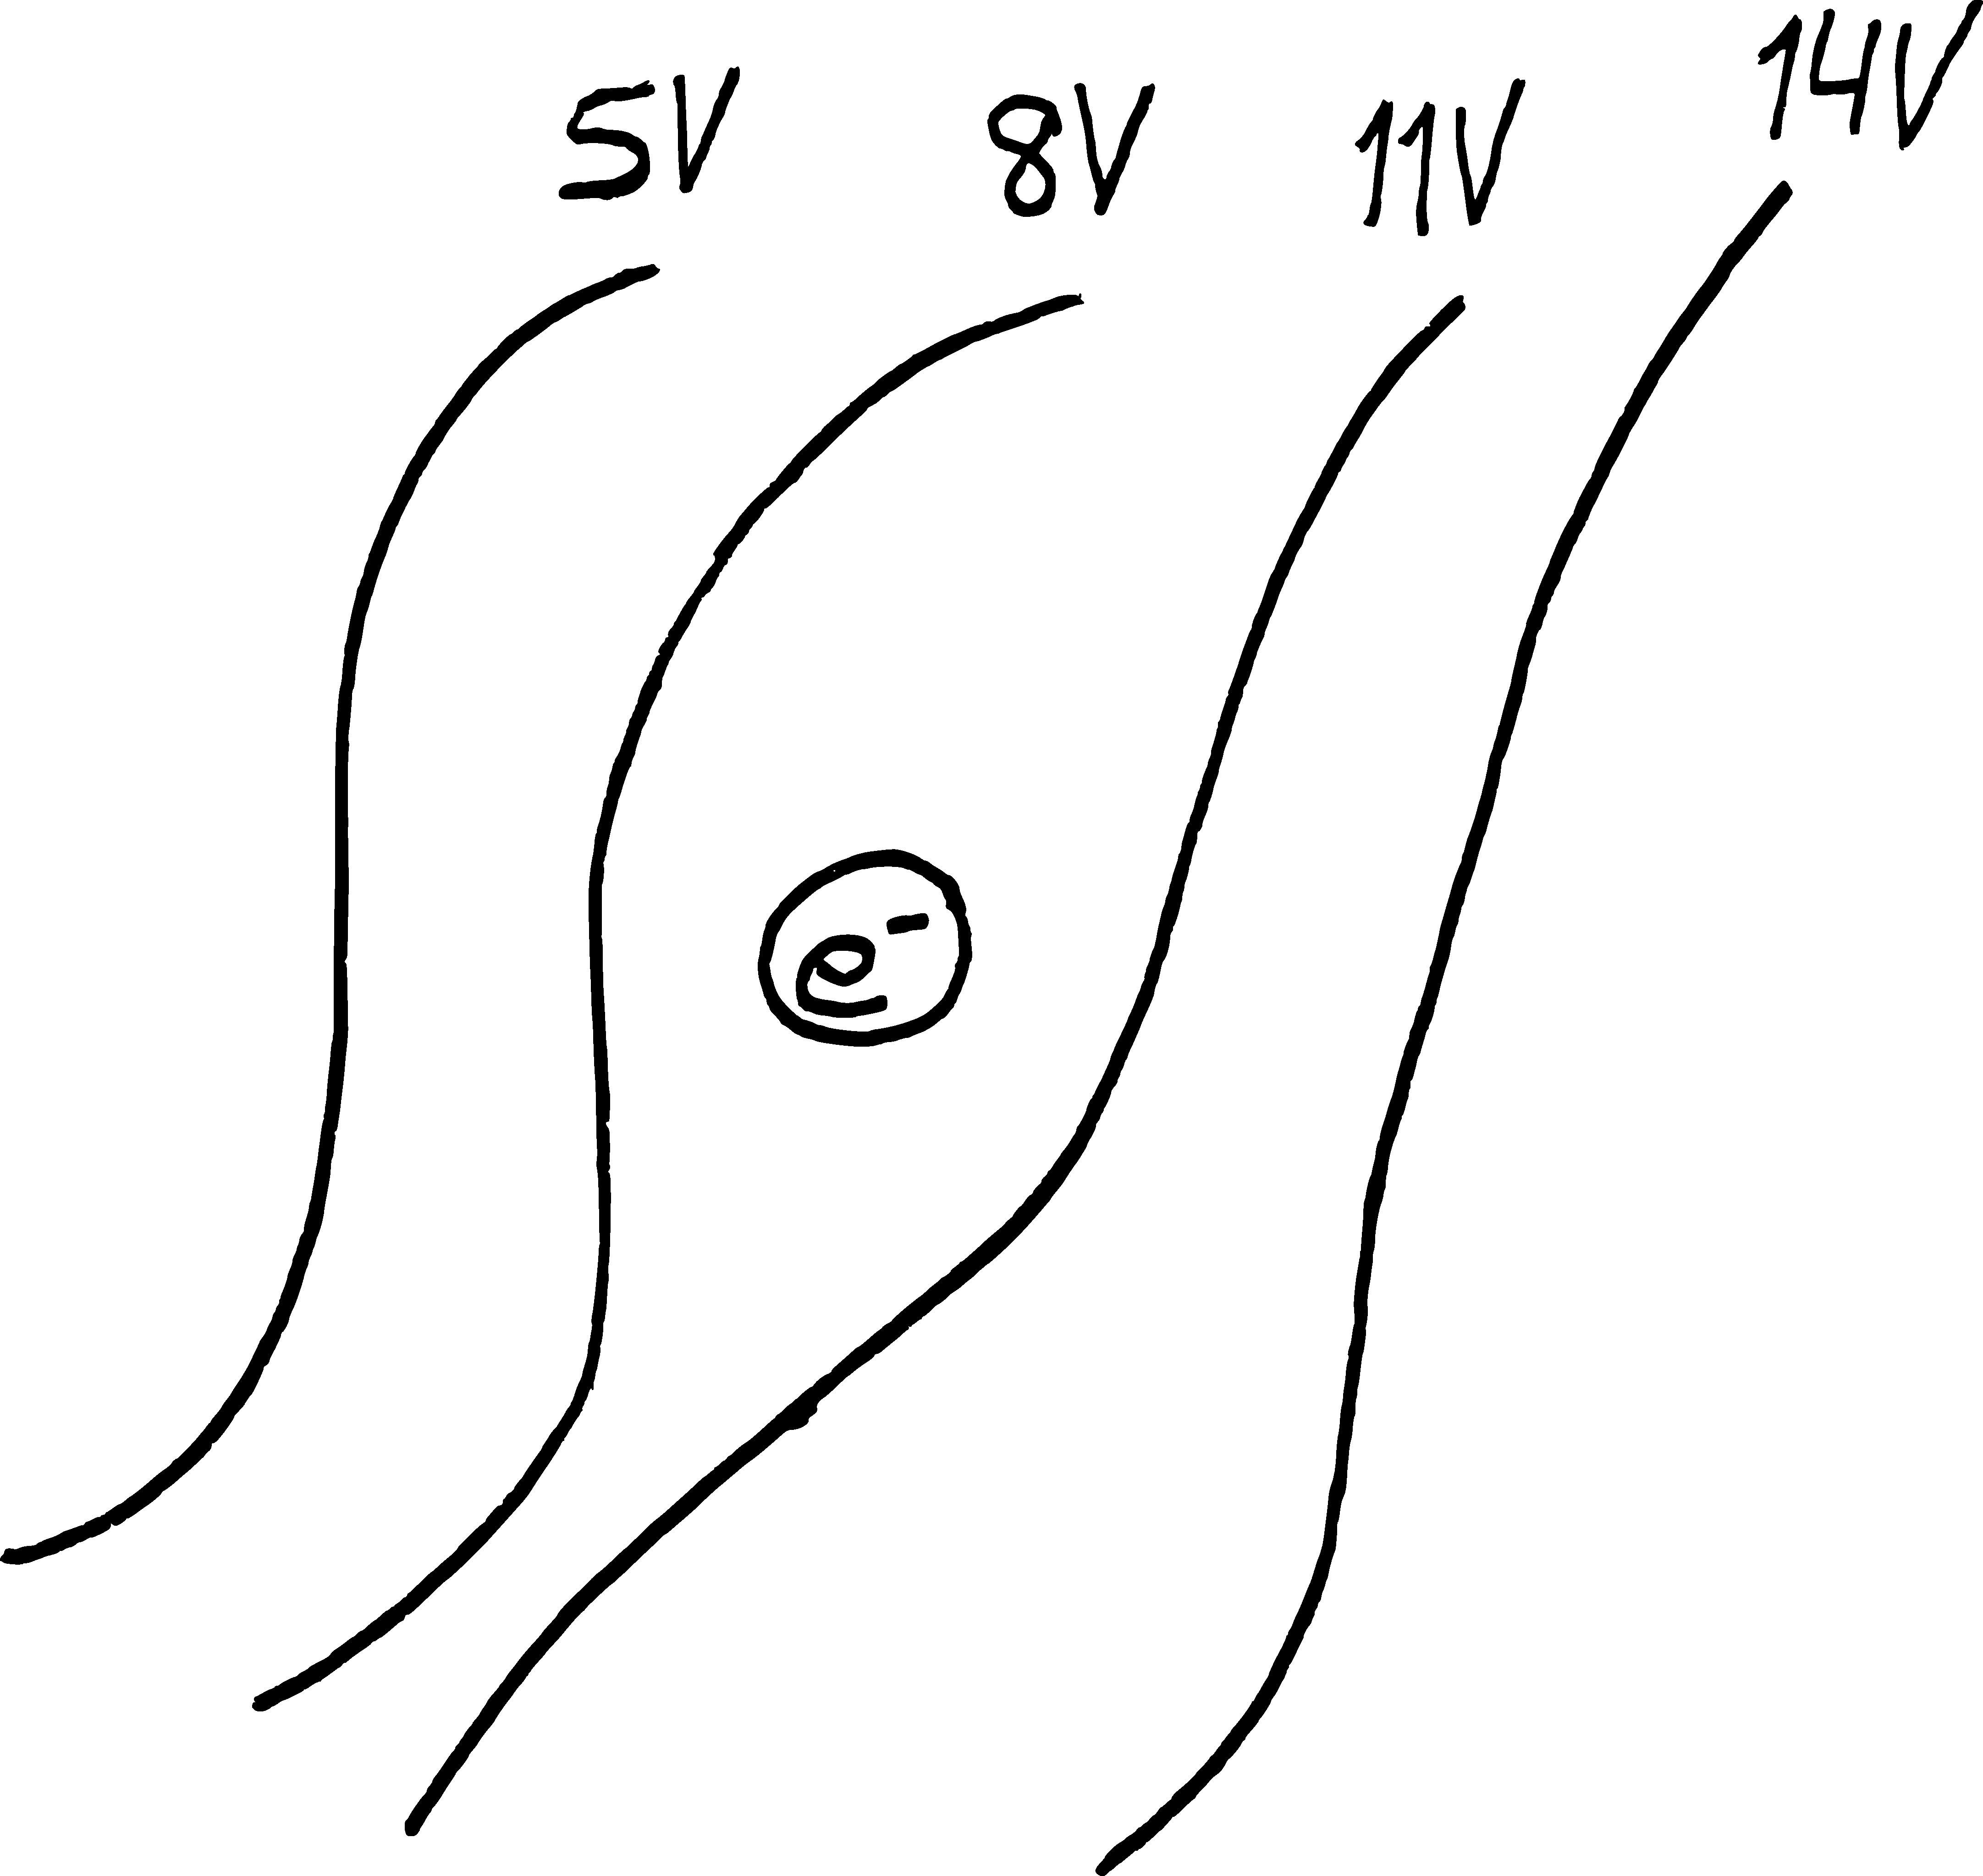
\includegraphics[width=5cm]{04-potentiel/figures/exercice-equipotentielles.pdf}
\end{center}

\begin{enumerate}
  \item Dans quelle direction est la force que subit l'électron?
  \item Tracez les lignes de champ électrique.
\end{enumerate}


\begin{center}
  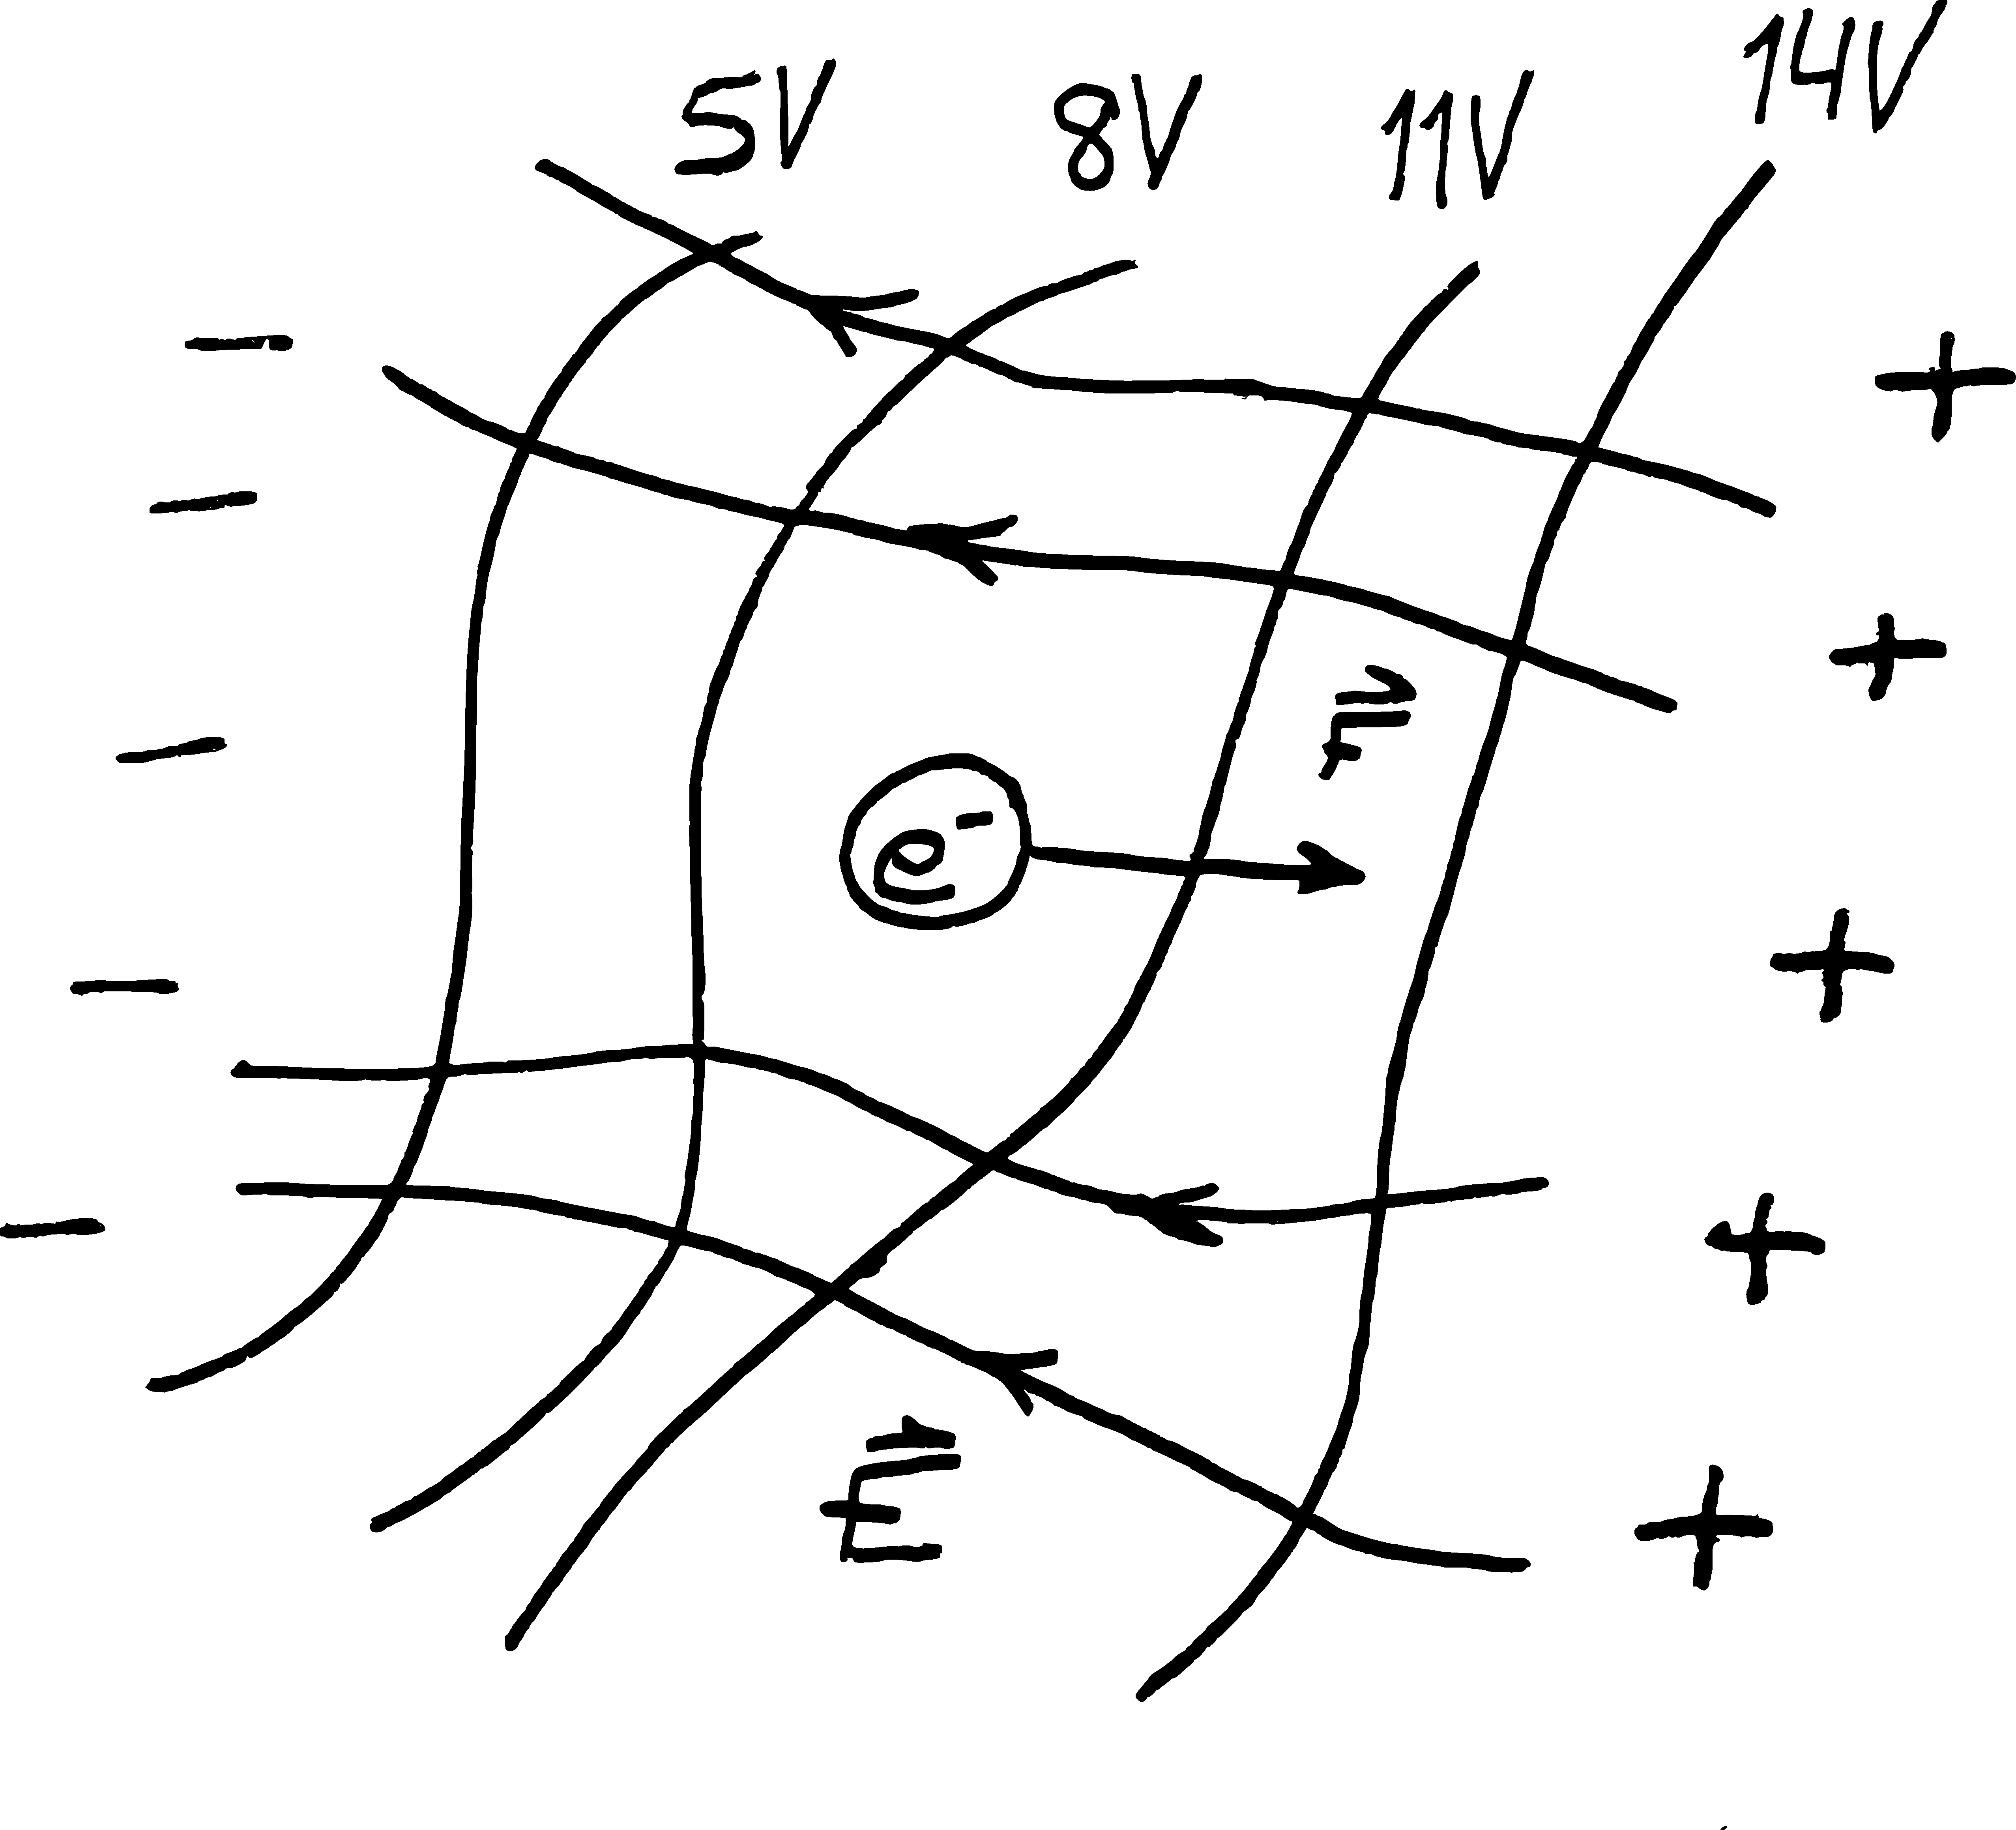
\includegraphics[width=5cm]{04-potentiel/figures/exercice-equipotentielles-solution.pdf}
\end{center}



Cet exercice permet de mettre en lumière quelques propriétés importantes des
équipotentielles et du potentiel électrique.

\begin{itemize}
  \item Plus les équipotentielles sont rapprochées les unes des autres, plus le
    champ électrique est grand à cet endroit.
  \item Les lignes de champ électrique vont des potentiels élevés vers les
    potentiels faibles.
  \item Une particule chargée négativement subira une force vers les potentiels
    élevés.
  \item Une particule chargée positivement subira une force vers les potentiels
    plus faibles.
\end{itemize}
